\documentclass{article}
\usepackage[paperwidth=18.5cm,paperheight=8.2cm,margin=0cm,noheadfoot]{geometry}
\usepackage{amsmath,amssymb}
\usepackage{tikz}
\usetikzlibrary{arrows.meta,positioning,calc,shadows.blur,backgrounds}
\usepackage{xcolor}
\pagestyle{empty}
\setlength{\parindent}{0pt}

% === Modern palette with gradient-friendly tones ===
\definecolor{deepblue}{HTML}{1A5276}
\definecolor{midblue}{HTML}{2E86C1}
\definecolor{lightblue}{HTML}{AED6F1}
\definecolor{softblue}{HTML}{D6EAF8}
\definecolor{bgblue}{HTML}{EBF5FB}

\definecolor{deeppurple}{HTML}{6C3483}
\definecolor{midpurple}{HTML}{8E44AD}
\definecolor{lightpurple}{HTML}{D2B4DE}
\definecolor{bgpurple}{HTML}{F4ECF7}

\definecolor{deeporange}{HTML}{BA4A00}
\definecolor{midorange}{HTML}{E67E22}
\definecolor{lightorange}{HTML}{F5CBA7}
\definecolor{bgorange}{HTML}{FEF5E7}

\definecolor{coralpink}{HTML}{E74C3C}
\definecolor{softcoral}{HTML}{FADBD8}
\definecolor{deepgray}{HTML}{2C3E50}
\definecolor{midgray}{HTML}{7F8C8D}
\definecolor{lightgray}{HTML}{D5D8DC}
\definecolor{panelbg}{HTML}{FAFCFE}

\begin{document}
\vspace*{0pt}\noindent
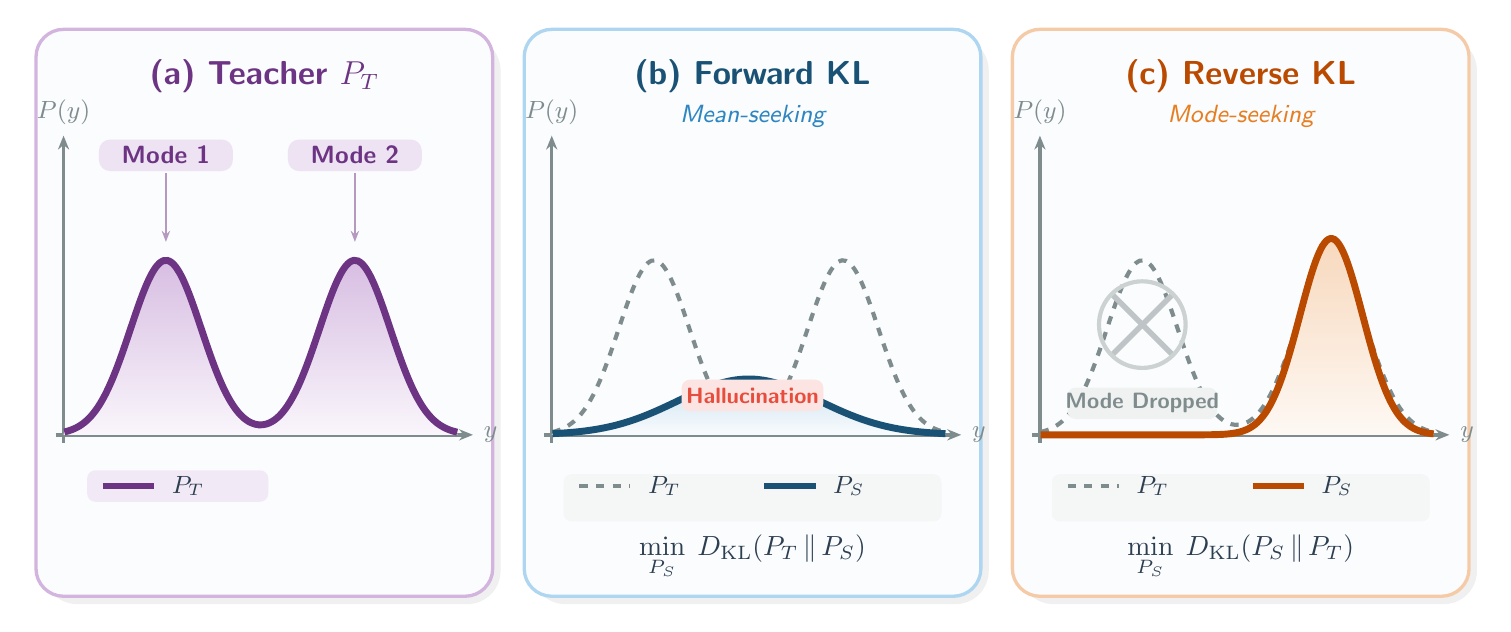
\begin{tikzpicture}[
    >=Stealth,
  ]

  % =================== Panel (a): Teacher P_T ===================
  % Card background with shadow
  \fill[black, opacity=0.06, rounded corners=12pt] 
    (-0.25, -2.15) rectangle (5.55, 5.05);
  \fill[panelbg, rounded corners=10pt] 
    (-0.35, -2.05) rectangle (5.45, 5.15);
  \draw[lightpurple, line width=1.2pt, rounded corners=10pt] 
    (-0.35, -2.05) rectangle (5.45, 5.15);

  \begin{scope}[shift={(0,0)}]
    % Title
    \node[font=\large\bfseries\sffamily, deeppurple] at (2.55, 4.55) {(a) Teacher $P_T$};
    
    % Axes — thick
    \draw[-{Stealth[length=5pt,width=4pt]}, line width=1.2pt, midgray] 
      (-0.1, 0) -- (5.2, 0) node[right, font=\small\sffamily, midgray] {$y$};
    \draw[-{Stealth[length=5pt,width=4pt]}, line width=1.2pt, midgray] 
      (0, -0.1) -- (0, 3.8) node[above, font=\small\sffamily, midgray] {$P(y)$};
    
    % Gradient fill under curve
    \shade[top color=midpurple!35, bottom color=midpurple!5, smooth, samples=100, domain=0.01:5]
      plot (\x, {2.5*(exp(-((\x-1.3)^2)/(2*0.45^2)) + exp(-((\x-3.7)^2)/(2*0.45^2)))/(0.45*sqrt(2*pi))})
      -- (5,0) -- (0,0) -- cycle;
    
    % Main curve — THICK
    \draw[deeppurple, line width=2.5pt, smooth, samples=100, domain=0.01:5]
      plot (\x, {2.5*(exp(-((\x-1.3)^2)/(2*0.45^2)) + exp(-((\x-3.7)^2)/(2*0.45^2)))/(0.45*sqrt(2*pi))});
    
    % Mode labels with pill badges
    \fill[midpurple!15, rounded corners=4pt] (0.45, 3.35) rectangle (2.15, 3.75);
    \node[font=\small\bfseries\sffamily, deeppurple] at (1.3, 3.55) {Mode 1};
    \fill[midpurple!15, rounded corners=4pt] (2.85, 3.35) rectangle (4.55, 3.75);
    \node[font=\small\bfseries\sffamily, deeppurple] at (3.7, 3.55) {Mode 2};
    
    % Arrows to peaks
    \draw[-{Stealth[length=4pt,width=3pt]}, deeppurple!50, line width=0.8pt] 
      (1.3, 3.32) -- (1.3, 2.45);
    \draw[-{Stealth[length=4pt,width=3pt]}, deeppurple!50, line width=0.8pt] 
      (3.7, 3.32) -- (3.7, 2.45);
    
    % Legend pill
    \fill[midpurple!12, rounded corners=3pt] (0.3, -0.85) rectangle (2.6, -0.45);
    \draw[deeppurple, line width=2pt] (0.5, -0.65) -- (1.15, -0.65);
    \node[font=\small\sffamily, deepgray, anchor=west] at (1.25, -0.65) {$P_T$};
  \end{scope}

  % =================== Panel (b): Forward KL ===================
  \fill[black, opacity=0.06, rounded corners=12pt] 
    (5.95, -2.15) rectangle (11.75, 5.05);
  \fill[panelbg, rounded corners=10pt] 
    (5.85, -2.05) rectangle (11.65, 5.15);
  \draw[lightblue, line width=1.2pt, rounded corners=10pt] 
    (5.85, -2.05) rectangle (11.65, 5.15);

  \begin{scope}[shift={(6.2,0)}]
    % Title
    \node[font=\large\bfseries\sffamily, deepblue] at (2.55, 4.55) {(b) Forward KL};
    \node[font=\small\itshape\sffamily, midblue] at (2.55, 4.05) {Mean-seeking};
    
    % Axes
    \draw[-{Stealth[length=5pt,width=4pt]}, line width=1.2pt, midgray] 
      (-0.1, 0) -- (5.2, 0) node[right, font=\small\sffamily, midgray] {$y$};
    \draw[-{Stealth[length=5pt,width=4pt]}, line width=1.2pt, midgray] 
      (0, -0.1) -- (0, 3.8) node[above, font=\small\sffamily, midgray] {$P(y)$};
    
    % Hallucination zone — soft coral gradient
    \shade[top color=coralpink!30, bottom color=coralpink!5, smooth, samples=60, domain=1.7:3.3]
      plot (\x, {1.6*exp(-((\x-2.5)^2)/(2*0.9^2))/(0.9*sqrt(2*pi))})
      -- (3.3, 0) -- (1.7, 0) -- cycle;
    
    % Teacher distribution — dashed gray, medium thickness
    \draw[midgray, line width=1.5pt, dashed, smooth, samples=100, domain=0.01:5]
      plot (\x, {2.5*(exp(-((\x-1.3)^2)/(2*0.45^2)) + exp(-((\x-3.7)^2)/(2*0.45^2)))/(0.45*sqrt(2*pi))});
    
    % Student gradient fill
    \shade[top color=midblue!25, bottom color=midblue!3, smooth, samples=100, domain=0.01:5]
      plot (\x, {1.6*exp(-((\x-2.5)^2)/(2*0.9^2))/(0.9*sqrt(2*pi))})
      -- (5,0) -- (0,0) -- cycle;
    
    % Student curve — THICK
    \draw[deepblue, line width=2.5pt, smooth, samples=100, domain=0.01:5]
      plot (\x, {1.6*exp(-((\x-2.5)^2)/(2*0.9^2))/(0.9*sqrt(2*pi))});
    
    % Hallucination label pill
    \fill[coralpink!15, rounded corners=3pt] (1.65, 0.3) rectangle (3.45, 0.7);
    \node[font=\footnotesize\bfseries\sffamily, coralpink] at (2.55, 0.5) {Hallucination};
    
    % Legend
    \fill[midgray!8, rounded corners=3pt] (0.15, -0.5) rectangle (4.95, -1.1);
    \draw[midgray, line width=1.5pt, dashed] (0.35, -0.65) -- (1.0, -0.65);
    \node[font=\small\sffamily, deepgray, anchor=west] at (1.1, -0.65) {$P_T$};
    \draw[deepblue, line width=2pt] (2.7, -0.65) -- (3.35, -0.65);
    \node[font=\small\sffamily, deepgray, anchor=west] at (3.45, -0.65) {$P_S$};
    
    % Formula
    \node[font=\normalsize, deepgray] at (2.55, -1.55) 
      {$\displaystyle\min_{P_S}\; D_{\mathrm{KL}}(P_T \,\|\, P_S)$};
  \end{scope}

  % =================== Panel (c): Reverse KL ===================
  \fill[black, opacity=0.06, rounded corners=12pt] 
    (12.15, -2.15) rectangle (17.95, 5.05);
  \fill[panelbg, rounded corners=10pt] 
    (12.05, -2.05) rectangle (17.85, 5.15);
  \draw[lightorange, line width=1.2pt, rounded corners=10pt] 
    (12.05, -2.05) rectangle (17.85, 5.15);

  \begin{scope}[shift={(12.4,0)}]
    % Title
    \node[font=\large\bfseries\sffamily, deeporange] at (2.55, 4.55) {(c) Reverse KL};
    \node[font=\small\itshape\sffamily, midorange] at (2.55, 4.05) {Mode-seeking};
    
    % Axes
    \draw[-{Stealth[length=5pt,width=4pt]}, line width=1.2pt, midgray] 
      (-0.1, 0) -- (5.2, 0) node[right, font=\small\sffamily, midgray] {$y$};
    \draw[-{Stealth[length=5pt,width=4pt]}, line width=1.2pt, midgray] 
      (0, -0.1) -- (0, 3.8) node[above, font=\small\sffamily, midgray] {$P(y)$};
    
    % Teacher distribution — dashed gray
    \draw[midgray, line width=1.5pt, dashed, smooth, samples=100, domain=0.01:5]
      plot (\x, {2.5*(exp(-((\x-1.3)^2)/(2*0.45^2)) + exp(-((\x-3.7)^2)/(2*0.45^2)))/(0.45*sqrt(2*pi))});
    
    % Student gradient fill
    \shade[top color=midorange!30, bottom color=midorange!5, smooth, samples=100, domain=0.01:5]
      plot (\x, {2.5*exp(-((\x-3.7)^2)/(2*0.4^2))/(0.4*sqrt(2*pi))})
      -- (5,0) -- (0,0) -- cycle;
    
    % Student curve — THICK
    \draw[deeporange, line width=2.5pt, smooth, samples=100, domain=0.01:5]
      plot (\x, {2.5*exp(-((\x-3.7)^2)/(2*0.4^2))/(0.4*sqrt(2*pi))});
    
    % Mode dropped — faded X with circle
    \draw[midgray!50, line width=2pt] (0.9, 1.0) -- (1.7, 1.8);
    \draw[midgray!50, line width=2pt] (0.9, 1.8) -- (1.7, 1.0);
    \draw[midgray!40, line width=1.5pt] (1.3, 1.4) circle (0.55);
    
    \fill[midgray!12, rounded corners=3pt] (0.35, 0.2) rectangle (2.25, 0.6);
    \node[font=\footnotesize\bfseries\sffamily, midgray] at (1.3, 0.4) {Mode Dropped};
    
    % Legend
    \fill[midgray!8, rounded corners=3pt] (0.15, -0.5) rectangle (4.95, -1.1);
    \draw[midgray, line width=1.5pt, dashed] (0.35, -0.65) -- (1.0, -0.65);
    \node[font=\small\sffamily, deepgray, anchor=west] at (1.1, -0.65) {$P_T$};
    \draw[deeporange, line width=2pt] (2.7, -0.65) -- (3.35, -0.65);
    \node[font=\small\sffamily, deepgray, anchor=west] at (3.45, -0.65) {$P_S$};
    
    % Formula
    \node[font=\normalsize, deepgray] at (2.55, -1.55) 
      {$\displaystyle\min_{P_S}\; D_{\mathrm{KL}}(P_S \,\|\, P_T)$};
  \end{scope}

\end{tikzpicture}
\end{document}
